\documentclass[11pt,a4paper]{article}
\usepackage[utf8]{inputenc}
\usepackage[T1]{fontenc}
\usepackage{amsfonts}
\usepackage[french]{babel}
\frenchbsetup{StandardLists=true} % à inclure si on utilise \usepackage[francais]{babel}
\usepackage{enumitem}
\usepackage{amssymb}
\usepackage{amsmath}
\usepackage{parskip}
\usepackage[left=2cm,right=2cm,top=2cm,bottom=2cm]{geometry}
\usepackage{multirow}
\usepackage[dvipsnames]{xcolor}

\usepackage[T1]{fontenc}
\usepackage{fouriernc}
\usepackage{graphicx}

\usepackage{setspace}
\singlespacing

\usepackage{pstricks}
\usepackage{xkeyval}
\usepackage{pst-labo}


\usepackage{multicol}
\usepackage{caption}
\usepackage{fancyhdr}
\pagestyle{fancy}
\renewcommand\headrulewidth{1pt}
\fancyhead[L]{Lycée Denis Diderot }
\fancyhead[R]{Classe de 1 Bac Pro }
\setcounter{page}{13}\fancyfoot[C]{page \thepage}
\fancyfoot[R]{Année 2024-2025}
\fancyfoot[L]{Alexis RUIZ}
\usepackage{multirow,tabularx,booktabs}
\newcommand{\cadreblanc}[1]{%
\medskip\framebox[\linewidth][c]{%
\rule{0mm}{#1mm}}\par
\medskip}

\usepackage{eurosym}

\usepackage{awesomebox}
\setlength{\aweboxvskip}{0mm}
\usepackage{pifont}
\usepackage{chemmacros}
\usepackage{chemist}
\chemsetup{modules=all}

\renewcommand{\arraystretch}{2}
\newcolumntype{C}[1]{>{\centering\arraybackslash }b{#1}}
\newcommand*\acocher{\quitvmode{\fboxsep0pt \fboxrule0.8pt \fbox{\vrule height1.8ex depth.1ex width0pt \vrule height0pt depth0pt width1.9ex }}}
\usepackage{colortbl}

\newcommand{\defproblem}{\awesomebox[black]{2pt}{\rotatebox{90}{\large{\textbf{Problématique}}}}{black}}
\newcommand{\defconclusion}{\awesomebox[black]{2pt}{\rotatebox{90}{\Large{\textbf{Conclusion}}}}{black}}
\newcommand{\defbox}{\awesomebox[black]{2pt}{
\includegraphics[scale=0.5]{images/appel exam.png}}{black}}


\frenchbsetup{StandardLists=true}



\begin{document}

\noindent

\begin{center}
\LARGE{Évaluation- Accélération et vitesse }\\[8mm]
\end{center}
\normalsize
\hrule 


\flushleft \textbf{NOM : \hfill Classe : \hspace{3cm} ~~\\[2mm]
Prénom:\\[0,4cm]
}
\hrule\
\\[0,2cm]

\vspace {8 mm}


\fbox{\textbf{Exercice 1 : Choisir la (ou les) bonne(s) réponse(s)}}


    \begin{tabular}{p{2mm} p{5.5cm}|C{3cm}|C{3cm}|C{3cm}}
    

        \ding{202} & L 'accélération s'exprime en :& $\Box $ ~~m/s & $\Box $ ~~km/h  & $\Box $ ~~$\mathrm{m/s^2}$ \\
         \hline
      \ding{203} & lors d'un mouvement rectiligne lorsque la vitesse diminue: & $\Box $ ~~l'accélération est négative & $\Box $ l'accélération est constante   & $\Box $ ~~ l'accélération est positive \\
        \hline
         \ding{204} & La vitesse se calcule grâce à la formule:  &$\Box $ ~~ $v=\dfrac{a}{t}$  &$\Box $ ~~ $v=a \times t$  & $\Box $ ~~$v=\dfrac{t}{a}$  \\
         \hline
         \ding{205} &Pour une distance de 40 m parcourue en 5 secondes: &$\Box $ ~~ $\mathrm{v=8 ~km/h}$  &$\Box $ ~~ $\mathrm{v=200 ~km/h}$  & $\Box $ ~~$\mathrm{v=8 ~m/s}$  \\

         \hline
         
        \ding{206} & Si je passe d'une vitesse de 5 m/s à une vitesse de 15 m/s en 2 secondes, mon accélération vaut:&$\Box $ ~~ $\mathrm{a=3 ~m/s^2}$  &$\Box $ ~~ $\mathrm{a=5 ~m/s^2}$  & $\Box $ ~~$\mathrm{a=10 ~m/s^2}$  \\

 
        
         \end{tabular}
\vspace{3mm}

\fbox{\textbf{Exercice 2 : Calculer une énergie}}

Un robot se déplace en suivant un mouvement rectiligne dont le cycle est décrit par le graphique suivant : 

\begin{enumerate}

\noindent%
\begin{minipage}{.50\textwidth}%

 \item Identifiez la nature du mouvement pour chacune des 3 phases. 

 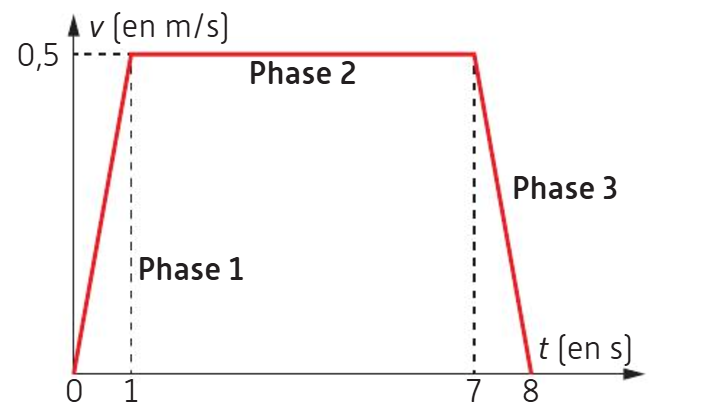
\includegraphics[width=\textwidth]{images/EX2.png}
 
\end{minipage}%
\hfill
\begin{minipage}{.40\textwidth}%
Phase 1 :\\
\cadreblanc{15}
Phase 2 :\\
\cadreblanc{15}
Phase 3 :\\
\cadreblanc{15}

\end{minipage}%

\item Calculer l'accélération, en $\mathrm{m/s^2}$ dans chaque cas. 

\begin{multicols}{3}

Phase 1 :\\
\cadreblanc{15}
Phase 2 :\\
\cadreblanc{15}
Phase 3 :\\
\cadreblanc{15}
    
\end{multicols}



 

    
\end{enumerate}

\newpage



\fbox{\textbf{Exercice 3 }} 
\begin{center}
    
\textbf{Quels sont les avantages de la voiture Rapida ? }


Les données ci-dessous sont des caractéristiques de deux automobiles. 


    

    \begin{tabular}{|>{\columncolor{orange!20}}p{4cm}||C{3cm}|C{3cm}|C{3cm}|}
         \hline
         Modèle & Rapida & Presto  \\
         \hline 
         Moteur &  Électrique &  Thermique   \\
         \hline
         Puissance  & 460 ch  &  384 ch   \\
         \hline 
         Consommation  & 10 kW/100 km   & 10 L/100 km   \\
         \hline 
         Rejet $\mathrm{CO_2}$  &  50 g/km &  240 g/km  \\
         \hline 
    \end{tabular}\end{center}
\begin{center}
    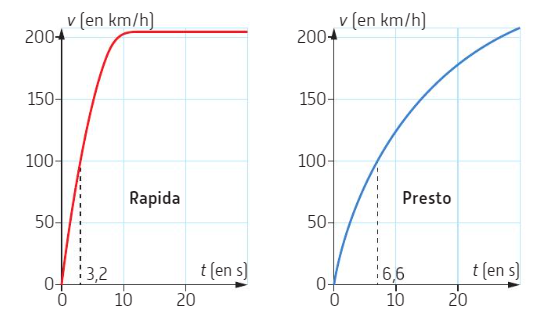
\includegraphics[scale=0.8]{images/courbes ex4.png}
\end{center}


\textbf{\ding{202} S'approprier} :

1.1 Quelle est la voiture qui, départ arrêté, atteint la première 50 km/h ? ~~100 km/h ? \\

\vspace{8mm}
\dotfill 

\vspace{8mm}
\dotfill 

\vspace{3mm}

1.2. Quelle est celle qui a une accélération constante jusqu'à 100 km/h ? 

\vspace{8mm}
\dotfill 

\vfill 



\textbf{\ding{203} Analyser - Raisonner} \\

Commentez les variations des deux courbes  modélisant la vitesse en fonction du temps entre 0 et 30s 

\begin{multicols}{2}
    Rapida : \\
    \cadreblanc{22}
    
    Presto : \\
    \cadreblanc{22}
    
\end{multicols}

\vfill 

\textbf{\ding{204} Réaliser} \\

Calculer l'accélération moyenne de chacun des deux véhicules pour passer de 0 à 100 km/h.  

\vspace{3mm}
\begin{multicols}{2}
    Rapida : \\
    \cadreblanc{30}
    
    Presto : \\
    \cadreblanc{30}
    
\end{multicols}


\vspace{3mm}



\textbf{\ding{205} Valider} \\

Un corps humain non entraîné supporte sans difficulté des accélérations horizontales inférieures à 1G. L'accélération d'un des deux véhicules dépasse-t-elle 1G (9,8 $\mathrm{m/s^2}$) entre 0 et 30 s. 

\cadreblanc{35}

\vfill 

\dotfill

\Large{Énigme : Bonus +1}

\dotfill

Dans la grille ci-dessous, numérotez les neuf cases de 1 à 9 de façon que dans n’importe quelle ligne, colonne et diagonale, on n’ait jamais deux entiers consécutifs.

Par exemple, 2 et 3 sont des entiers consécutifs. 2 et 4 ne le sont pas.
\begin{center}
   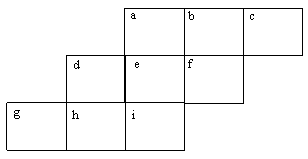
\includegraphics[]{controleenigme.png} 
\end{center}

  \vfill 
  

\end{document}